%! TEX root = ../main.tex
\documentclass[main]{subfiles}

\begin{document}
\section{表面繊維}

カーリングブラシパッドの表面性状を観察するにあたって,表面繊維の状態が使用するごとにどれほど摩耗しているかを
デジタルマイクロスコープを用いて調査した.デジタルマイクロスコープは100倍~1000倍まで見ることができるも
のを使用した.それぞれのサンプルで、一番汚れている縁の部分(下図の赤枠)と汚れが少ない中心部分
(下図の黒枠)を撮影した.10~15投使用したものと長期間使用したものはサンプルを2つずつ用意した.
10~15投使用したものに関しては,左右偏りなく使用されているもの(A)と片方に使用具合が偏って
いるもの(B)を用意した.
具体的には下記の項目どおりである.

\begin{itemize}
    \item 未使用×1
    \item 10~15投使用×2
    \item 長時間使用×2
\end{itemize}

\begin{figure}[htbp]
    \centering
    \begin{subfigure}[htbp]{0.3\linewidth}
        \centering
        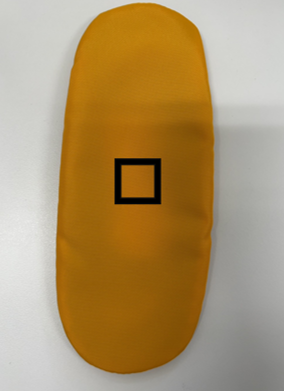
\includegraphics[keepaspectratio, width=0.8\linewidth, height=\linewidth]{figures/caring_brush_pad/misiyou.png}
        \caption{未使用}
        \label{fig:label}
    \end{subfigure}
    \begin{subfigure}[htbp]{0.3\linewidth}
        \centering
        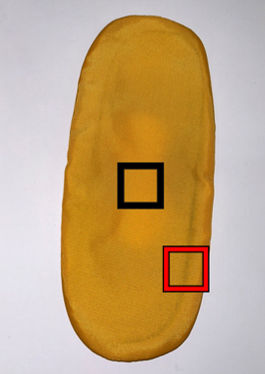
\includegraphics[keepaspectratio, width=0.8\linewidth, height=\linewidth]{figures/caring_brush_pad/10~15A.png}
        \caption{10~15投使用A}
        \label{fig:label}
    \end{subfigure}
    \begin{subfigure}[htbp]{0.3\linewidth}
        \centering
        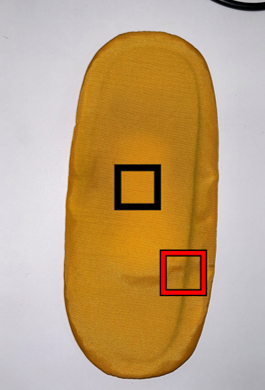
\includegraphics[keepaspectratio, width=0.8\linewidth, height=\linewidth]{figures/caring_brush_pad/10~15B.png}
        \caption{10~15投使用B}
        \label{fig:label}
    \end{subfigure}
    \begin{subfigure}[htbp]{0.3\linewidth}
        \centering
        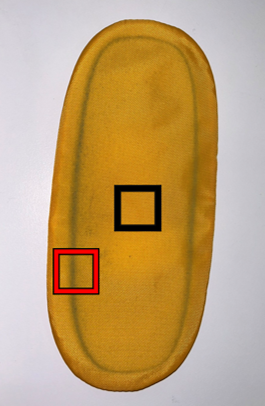
\includegraphics[keepaspectratio, width=0.8\linewidth, height=\linewidth]{figures/caring_brush_pad/chouki.png}
        \caption{長期使用A}
        \label{fig:label}
    \end{subfigure}
    \begin{subfigure}[htbp]{0.3\linewidth}
        \centering
        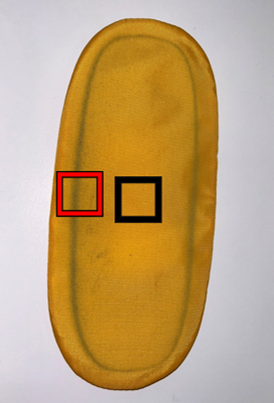
\includegraphics[keepaspectratio, width=0.8\linewidth, height=\linewidth]{figures/caring_brush_pad/choukiB.png}
        \caption{長期使用B}
        \label{fig:label}
    \end{subfigure}
\end{figure}


\end{document}